\begin{frame}
    \titlepage
\end{frame}

\begin{frame}{logistics: TRICKY}
    \begin{itemize}
    \item HW assignment out
    \item ``infecting'' an executable
    \end{itemize}
\end{frame}

\begin{frame}{last time}
    \begin{itemize}
    \item anti-virus:
    \begin{itemize}
        \item heuristic: malware messing up executables?
            \begin{itemize}
            \item key idea: wrong segment of executable?
            \item switching segments of the executable?
            \item weird API calls/names
            \end{itemize}
        \item detecting bad behavior?
    \end{itemize}
    \item anti-anti-virus
        \begin{itemize}
        \item ``encrypted'' data
        \item ``encrypted'' code: ``packers''
        \item oligomorphic and polymorphic: changing \myemph{``encrypters''}
        \end{itemize}
    \end{itemize}
\end{frame}

\begin{frame}{today}
    \begin{itemize}
    \item this time:
        \begin{itemize}
        \item metamorphic: changing encrypter \myemph{and body}
        \end{itemize}
    \item also: more anti-anti-virus
        \begin{itemize}
        \item anti-virtualization review
        \item anti-debugging
        \item \ldots
        \end{itemize}
    \end{itemize}
\end{frame}

\section{anti-virus techniques}

\subsection{review: pattern matching}

\begin{frame}[fragile,label=reCheat]{regular expression cheatsheet}
    \begin{itemize}
    \item {\tt a} --- matches {\tt a}
    \item {\tt a*} --- matches \textit{(empty string)}, {\tt a}, {\tt aa}, {\tt aaa}, \ldots
    \item {\tt a\textbackslash*} --- matches the string {\tt a*}
    \item {\tt foo|bar} --- matches {\tt foo}, {\tt bar}
    \item {\tt [ab]} --- matches {\tt a}, {\tt b}
    \item \verb|[^ab]| --- matches any byte except a and b
    \item {\tt (foo|bar)*} ---
        \begin{itemize}
        \item \textit{(empty string)}, {\tt foo}, {\tt bar}, {\tt foobar}, {\tt barfoo}, \ldots
        \end{itemize}
    \item {\tt (.|\textbackslash{}n)*} --- matches anything whatsoever
    \end{itemize}
\end{frame}

\begin{frame}{upcoming assignment: LEX}
    \begin{itemize}
    \item use {\tt flex} to write a scanner for the pattern:
        \begin{itemize}
        \item {\tt push \$0x12345678; ret}
        \end{itemize}
    \item explain a false positive, propose practical solution
    \end{itemize}
\end{frame}

\subsubsection{polymorphic case study: 1260}

\begin{frame}[fragile,label=v1260]{example: 1260 (virus)}
\lstset{
    style=small,
    language=myasm,
    moredelim={**[is][\btHL<2-3|handout:0>]{@hi2@}{@endhi@}},
    moredelim={**[is][\btHL<4-5|handout:0>]{@hi3@}{@endhi@}},
}
% FIXME: adapt Listing 7.5
\begin{tabular}{ll}
\begin{lstlisting}
    @hi2@inc %si@endhi@
    mov @hi3@$0x0e9b@endhi@, %ax
    @hi2@clc@endhi@
    mov $0x12a, %di
    @hi2@nop@endhi@
    mov $0x571, %cx
decrypt:
    xor %cx, (%di)
    @hi2@sub %dx, %bx@endhi@
    @hi2@sub %cx, %bx@endhi@
    @hi2@sub %ax, %bx@endhi@
    @hi2@nop@endhi@
    @hi2@xor %cx, %dx@endhi@
    xor %ax, (%di)
    ...
\end{lstlisting}
&
\begin{lstlisting}
    mov @hi3@$0x0a43@endhi@, %ax
    @hi2@nop@endhi@
    mov $0x15a, %di
    @hi2@sub %dx, %bx@endhi@
    @hi2@sub %cx, %bx@endhi@
    mov $0x571, %cx
    @hi2@clc@endhi@
decrypt:
    xor %cx, (%di)
    @hi2@xor %cx, %dx@endhi@
    @hi2@sub %cx, %bx@endhi@
    @hi2@nop@endhi@
    @hi2@xor %cx, %bx@endhi@
    xor %ax, (%di)
    ...
\end{lstlisting}
\end{tabular}
\imagecredit{adapted from Szor, Listing 7.5}
\end{frame}

\begin{frame}[fragile,label=multVers]{multiple versions?}
    \begin{itemize}
    \item in ``encrypted'' code:
    \end{itemize}
\lstset{language=C,style=small}
\begin{lstlisting}
void generateDecrypter() {
    int key = random();
    writeRandomNop();
    if (random()) {
        writeMovKey(key);
        writeMovCodeLoc();
    } else {
        writeMovCodeLoc();
        writeMovKey(key);
    }
    writeRandomNop();
    ...
}
\end{lstlisting}
\end{frame}

\begin{frame}{typical polymorphic malware layout}
\begin{tikzpicture}
\draw[very thick] (0, 0) rectangle (6, -7);
\draw[thick,fill=blue!20] (0, 0) rectangle (6, -2) node[midway,font=\large] { decrypter };
\draw[thick,pattern color=red,pattern=north west lines] (0, -2) rectangle (6, -7);
\node[anchor=center,font=\large,fill=white,draw=red] at (3, -4) { ``encrypted'' code };
\draw[thick,fill=green!40] (2, -5) rectangle (4, -6);
\node[fill=white,anchor=north,draw=green] at (3, -6) {
    decrypter generator code
};
\draw[very thick,decoration=brace,decorate] (6.125, -2) -- (6.125, -7);
\node[anchor=west,align=left] at (6.25, -4.5) { unchanged when copied \\ 
        except re-``encrypted''};
\draw[very thick,decoration=brace,decorate] (6.125, 0) -- (6.125, -2);
\node[anchor=west,align=left] at (6.25, -1) { generated from template \\
in ``encrypted'' part };
\end{tikzpicture}
\end{frame}

\begin{frame}{polymorphic/oligomorphic}
    \begin{itemize}
    \item \myemph{only ``encrypter'' changes}
    \item ``encrypted'' code to generate encrypter
    \item only need to handle what encrypter does
    \item simplest version: just have several versions in encrypted code
    \item second simplest version: template with holes
    \item \myemph{never need to read machine code!}
    \end{itemize}
\end{frame}


\begin{frame}{common theme: run it and see}
    \begin{itemize}
    \item behavior-based detection:
        \begin{itemize}
        \item detect modifications to system files
        \end{itemize}
    \item defeating encrypters
        \begin{itemize}
        \item run encrypter, look for results
        \end{itemize}
    \vspace{.5cm}
    \item often requires VM
    \item \textbf{much} slower than pattern matching
    \item has its own countermeasures
    \end{itemize}
\end{frame}

\begin{frame}{on goats}
    \begin{itemize}
    \item analysis --- and maybe detection --- uses \textit{goat files}
    \item ``\myemph{sacrificial goat}'' to get changed by malware
    \vspace{.5cm}
    \item easier to look for than patterns in memory?
    \end{itemize}
\end{frame}

\begin{frame}{goats as detection}
    \begin{itemize}
    \item tripwire for malware
    \item touching do-nothing {\tt .exe} --- very likely bad
    \end{itemize}
\end{frame}

\begin{frame}{goats as analysis}
    \begin{itemize}
    \item more important for analysis of \myemph{changing malware}
    \item want examples of \myemph{multiple versions}
    \item want it to be obvious where malware code added
        \begin{itemize}
        \item e.g. big cavities to fill in original
        \item e.g. obvious patterns in original code/data
        \end{itemize}
    \end{itemize}
\end{frame}

\begin{frame}{on avoiding goats}
    \begin{itemize}
    \item heuristics can avoid simple goat files, e.g.:
        \begin{itemize}
        \item don't infect small programs
        \item don't infect huge programs
        \item don't infect programs with huge amounts of {\tt nop}s
        \item \ldots
        \end{itemize}
    \end{itemize}
\end{frame}

\section{heuristics for detecting packers}

\begin{frame}<1>[label=findingPackers]{finding packers}
    \begin{itemize}
    \item easiest way to decrypt self-decrypting code --- run it!
    \item solution: \myemph<1>{virtual machine} in antivirus software
    \vspace{.5cm}
    \item makes \myemph<2>{antivirtualization/emulation} more important
    \end{itemize}
\end{frame}

\begin{frame}{finding packers with VM}
    \begin{itemize}
    \item run program in VM for a while
        \begin{itemize}
        \item how long?
        \end{itemize}
    \item then scan memory for \myemph{known patterns}
    \item defeats \myemph{entire ``strategy''}
    \end{itemize}
\end{frame}

\subsection{DEP}

\begin{frame}{stopping packers}
    \begin{itemize}
    \item it's \myemph<2>{unusual} to jump to code you wrote
    \item modern OSs: memory is executable \textit{or} writable 
    \item very rarely executable and writeable
    \end{itemize}
\end{frame}

\begin{frame}{diversion: DEP/{\tt W\textasciicircum X}}
    \begin{itemize}
    \item memory executable or writeable --- but not both
    \item exists for \myemph{exploits} (later in course), not packers
    \item requires hardware support to be fast (\myemph{early 2000s+})
    \item various names for this feature:
        \begin{itemize}
        \item Data Execution Prevention (DEP) (Windows)
        \item {\tt W\textasciicircum X} (``write XOR execute'')
        \item NX/XD/XN bit  (underlying hardware support)
            \begin{itemize}
            \item (No Execute/eXecute Disable/eXecute Never)
            \end{itemize}
        \end{itemize}
    \item \myemph{system calls} needed to switch modes 
    \end{itemize}
\end{frame}

\begin{frame}{unusual, but\ldots}
    \begin{itemize}
    \item binary translation
        \begin{itemize}
        \item convert machine code to new machine code at runtime
        \end{itemize}
    \item Java virtual machine, JavaScript implementations
        \begin{itemize}
        \item ``just-in-time'' compilers
        \end{itemize}
    \item dynamic linkers
        \begin{itemize}
        \item load new code from a file --- same as writing code?
        \end{itemize}
    \item those packed commercial programs
    \vspace{.5cm}
    \item programs need to \myemph{explicitly} ask for write+exec
    \end{itemize}
\end{frame}

\section{antivirtualization}

\againframe<2>{findingPackers}

\begin{frame}{recurring theme}
    \begin{itemize}
    \item don't \myemph{analyze code} --- just run it!
    \vspace{.5cm}
    \item avoids the halting problem, kinda
    \item doesn't matter how much effort spent writing decrypters, etc.
    \end{itemize}
\end{frame}

\begin{frame}<1>[label=antivirtIndex]{antivirtualization techniques}
    \begin{itemize}
    \item \myemph<2>{query virtual devices}
        \begin{itemize}
        \item<3> solution: mirror devices of some real machine
        \end{itemize}
    \item \myemph<4>{time operations that are slower in VM/emulation}
        \begin{itemize}
        \item<5> solution: virtual clock
        \end{itemize}
    \item \myemph<6>{use operations not supported by VM}
        \begin{itemize}
        \item<7> solution: support everything
        \end{itemize}
    \end{itemize}
\end{frame}

\againframe<2>{antivirtIndex}

\begin{frame}{virtual devices}
    \begin{itemize}
    \item VirtualBox device drivers?
    \item VMware-brand ethernet device?
    \item \ldots
    \end{itemize}
\end{frame}

\againframe<3-4>{antivirtIndex}

\begin{frame}{slower operations}
    \begin{itemize}
    \item not-``native'' VM:
        \begin{itemize}
        \item i.e., emulation or binary translation
        \item everything is really slow
        \end{itemize}
    \item otherwise --- trigger ``callbacks'' to VM implementation:
        \begin{itemize}
        \item system calls?
        \item allocating and accessing memory?
        \end{itemize}
    \item \ldots and hope it's reliably slow enough
    \end{itemize}
\end{frame}


\againframe<5-6>{antivirtIndex}

\begin{frame}{operations not supported}
    \begin{itemize}
    \item missing instructions?
        \begin{itemize}
        \item FPU instructions
        \item MMX/SSE instructions
        \item undocumented (!) CPU instructions
        \end{itemize}
    \item not handling OS\tikzmark{OS} features?
        \begin{itemize}
        \item setting up special handlers for segfault
        \item multithreading
        \item system calls that make callbacks
        \item \ldots
        \end{itemize}
    \end{itemize}
    \begin{tikzpicture}[overlay,remember picture]
        \begin{visibleenv}<2->
        \node[mycallout=OS,align=center,anchor=center] at ([yshift=-3cm]current page.center) {
            antivirus not running system VM to do decryption \\
            needs to emulate lots of the OS itself
        };
        \end{visibleenv}
    \end{tikzpicture}
\end{frame}

\begin{frame}{attacking virtualization patience}
    \begin{itemize}
    \item looking for unpacked virus in VM
    \item \ldots or other malicious activity
    \item when are you done looking?
    \vspace{.5cm}
    \item<2-> malware solution: \myemph<2>{take too long}
        \begin{itemize}
        \item not hard if virtualization uses ``slow'' implementation
        \vspace{.25cm}
        \item slow? maybe allows more inspection of program
        \item (e.g. switching segments, newly written code)
        \end{itemize}
    \item<3-> malware solution: \myemph<3>{don't infect consistently}
    \end{itemize}
\end{frame}

\begin{frame}[fragile,label=prob]{probability}
\lstset{language=C,style=smaller}
    \begin{tikzpicture}
    \node[draw,align=center] (malware) {
\begin{lstlisting}
if (randomNumber() == 4) {
    unpackAndRunEvilCode();
}
\end{lstlisting}
    };
    \node[draw=red,very thick,align=left,above right=1cm of malware] (avCase1) {
        antivirus emulator: \\
        \lstinline|randomNumber() == 3| \\
        \textbf{\color{green!60!black}looks clean!}
    }; 
    \node[draw,align=left,right=1cm of malware]  (avCase2) {
        real execution \#1: \\
        \lstinline|randomNumber() == 2| \\
        \textbf{\color{green!60!black}no infection!}
    }; 
    \node[draw,align=left,below right=1cm and 0cm of malware] (avCase3) {
        real execution \#$N$: \\
        \lstinline|randomNumber() == 4| \\
        \textbf{\myemph{infect!}}
    }; 
    \node at ($(avCase2)!0.5!(avCase3)$) {\ldots};
    \draw[ultra thick,dashed,-Latex] (malware) -- (avCase1.west);
    \draw[ultra thick,dashed,-Latex] (malware) -- (avCase2.west);
    \draw[ultra thick,dashed,-Latex] (malware) -- (avCase3.west);
    \end{tikzpicture}
\end{frame}


\section{metamorphic virsues}

\begin{frame}{signatures in RAM}
\begin{tikzpicture}
\node[anchor=south] at (2, 0) { on disk };
\draw[very thick] (0, 0) rectangle (4, -7);
\draw[thick,fill=blue!20] (0, 0) rectangle (4, -2) node[midway,font=\large] { decrypter };
\draw[thick,pattern color=red,pattern=north west lines] (0, -2) rectangle (4, -7);
\node[anchor=center,fill=white,draw=red,align=center] at (2, -4) { ``encrypted'' \\ code };

\draw[-Latex,ultra thick] (4.25, -3.5) -- (5.75, -3.5);

\node[anchor=south] at (8, 0) { in memory (after a while) };
\draw[thick,fill=blue!20] (6, 0) rectangle (10, -2) node[midway,font=\large] { decrypter };
\draw[thick] (6, -2) rectangle (10, -7);
\node[anchor=center,align=center] at (8, -4) { decrypted code \\ (\textbf{good signature})};
\end{tikzpicture}
\end{frame}

\begin{frame}{changing bodies}
    \begin{itemize}
    \item ``decrypting'' a virus body gives body for ``signature''
        \begin{itemize}
        \item ``just'' need to run decrypter
        \end{itemize}
    \item how about avoiding static signatures entirely
    \item called \myemph{metamorphic}
        \begin{itemize}
        \item versus \myemph{polymorphic} --- only change ``decrypter''
        \end{itemize}
    \end{itemize}
\end{frame}

\begin{frame}{metamorphic versus polymorphic}
    \begin{itemize}
    \item big change in difficulty
    \item polymorphic: can have ``template'' with blanks
    \item metamorphic: probably \myemph{``understand'' machine code}
        \begin{itemize}
        \item could have been doing this with polymorphic, but probably not
        \end{itemize}
    \end{itemize}
\end{frame}

\begin{frame}[fragile,label=regSwap]{example: changing bodies}
\lstset{language=myasm,style=smaller}
\begin{tabular}{ll}
\begin{lstlisting}
pop %edx
mov $0x4h, %edi
mov %ebp, %esi
mov $0xC, %eax
add $0x88, %edx
mov (%edx), %ebx
mov %ebx, 0x1118(%esi,%eax,4)
\end{lstlisting}
&
\begin{lstlisting}
pop %eax
mov $0x4h, %ebx
mov %ebp, %esi
mov $0xC, %edi
add $0x88, %eax
mov (%eax), %esi
mov %esi, 0x1118(%esi,%eax,4)
\end{lstlisting}
\end{tabular}
\begin{onlyenv}<1>
\begin{itemize}
\item \myemph{every instruction} changes
\item likely with \myemph{machine code parser!}
    \begin{itemize}
    \item locate register number bits
    \item swap register numbers w/table lookup
    \end{itemize}
\end{itemize}
\end{onlyenv}
\begin{onlyenv}<2>
\begin{itemize}
\item still has good signatures
    \begin{itemize}
    \item with \myemph{alternatives} for each possible register selection
    \end{itemize}
\item but harder to write/slower to match
    \begin{itemize}
    \item in addition to running VM to decrypt
    \end{itemize}
\end{itemize}
\end{onlyenv}
\end{frame}

\subsection{Evol example}

% FIXME
\begin{frame}<1>[fragile,label=caseEvol]{case study: Evol}
    \begin{itemize}
    \item via Lakhatia et al, ``Are metamorphic viruses really invincible?'', Virus Bulletin, Jan 2005.
    \item ``\myemph{mutation engine}''
        \begin{itemize}
        \item run as part of propagating the virus
        \end{itemize}
    \end{itemize}
    \begin{tikzpicture}
        \tikzset{
            every node/.style={font=\small,align=center},
            hiOn/.style={alt=<#1>{red,ultra thick}{}},
        }
        \path node[draw,hiOn=2] (disasm) {disassemble} -- ++(2.5cm,0) node (lens) {instr. \\ lengths} -- ++(2cm,0) node[draw,hiOn=3] (xform) {transform}
              -- ++(2.5cm,0) node[draw,hiOn=4] (reloc) {relocate};
        \node (origCode) at ([xshift=-2cm,yshift=1cm]disasm.north) {code};
        \node (finalCode) at ([xshift=2cm,yshift=-1cm]reloc.south) {code};
        \begin{scope}[thick,-Latex]
        \draw (origCode) |- (disasm);
        \draw (disasm) -- (lens);
        \draw (lens) -- (xform);
        \draw (xform) -- (reloc);
        \draw (reloc) -| (finalCode);
        \end{scope}
    \end{tikzpicture}
\end{frame}

\againframe<2>{caseEvol}

\begin{frame}{Evol instruction lengths}
    \begin{itemize}
    \item sounds really complicated?
        \begin{itemize}
        \item instruction prefixes, ModRM byte parsing, \ldots
        \item big table of opcodes?
        \end{itemize}
    \item virus only handles instructions it has:
        \begin{itemize}
        \item about 61 opcodes, 32 of them identified by first four bits
        \item (opcode {\tt 0x7\textit{x}} -- conditional jump)
        \end{itemize}
    \item no prefixes, no floating point
    \item only {\tt \%reg} or {\tt \$constant} or {\tt offset(\%reg)}
    \end{itemize}
\end{frame}

\againframe<3>{caseEvol}

\begin{frame}[fragile,label=evolXform]{Evol transformations}
\lstset{language=myasm,style=small}
    \begin{itemize}
    \item some stuff left alone
    \item static or random one of $N$ transformations
    \item example:
    \end{itemize}
\begin{tikzpicture}
\tikzset{
    every node/.style={font=\small,align=center}
}
\node[draw] (movebpEight) {
\begin{lstlisting}
mov %eax, 8(%ebp)
\end{lstlisting}
};

\node[draw,right=2cm of movebpEight] (movebpExpand) {
\begin{lstlisting}
push %ecx
mov %ebp, %ecx
add $0x12, %ecx
mov %eax, -0xa(%ecx)
pop %ecx
\end{lstlisting}
};
\node[anchor=north east] at ([yshift=-.25cm]movebpExpand.south east) {
    uses more stack space --- save temporary \\
    code gets \myemph{bigger each time}
};
\end{tikzpicture}
\imagecredit{Lakhotia et al., ``Are metamorphic viruses really invincible?'', Virus Bulletin, Jan 2005}
\end{frame}

\againframe<4>{caseEvol}

\begin{frame}{mutation with relocation}
    % FIXME: XXX
    \begin{itemize}
    \item table mapping old to new locations
        \begin{itemize}
        \item list of number of bytes generated by each transformation
        \end{itemize}
    \item list of locations references in original
        \begin{itemize}
        \item record relative offset in jump
        \item record absolute offset in original
        \end{itemize}
    \end{itemize}
\end{frame}

\begin{frame}[fragile,label=relocEx]{relocation example}
\lstset{language=myasm,style=small}
\begin{tikzpicture}
\node (code) {
\begin{lstlisting}
    mov ...
    mov ...
0x9:
    xor %rax, (%rbx)
    inc %rbx
    dec %rcx
    jne 0x9
\end{lstlisting}
};
\begin{visibleenv}<2->
\matrix[tight matrix,nodes={font=\small},anchor=north west,
    nodes={font=\tt,text width=2cm,text depth=.1mm,minimum height=.4cm},
    row 1/.style={nodes={font=\small\bfseries,minimum height=1cm}},
    column 1/.style={text=blue!60!black,nodes={text width=1.75cm}},
    column 2/.style={text=green!60!black},
    column 3/.style={nodes={text width=1.1cm,font=\small\tt}},
    column 4/.style={nodes={text width=1.3cm,font=\small\tt,draw=none}},
    label={[font=\small]north:table from transformation},
] (lensTable) at ([xshift=0cm]code.north east) {
    orig. loc \& new loc \& addr \& ~ \\
    5 \& 10 \& -- \& mov \\
    7 \& 13 \& -- \& mov \\
    |[red]|\textbf{9} \& 20 \& -- \& xor \\
    10 \& 21 \& -- \& inc \\
    11 \& 26 \& -- \& dec \\
    14 \& 29 \& |[red]| \textbf{9} \& jne \\
};
\end{visibleenv}
\begin{visibleenv}<3->
\matrix[tight matrix,nodes={font=\fontsize{9}{10}\selectfont,minimum height=1.2cm},anchor=north west,
    nodes={font=\tt,text width=3cm},
    row 1/.style={nodes={font=\small\bfseries,minimum height=0.7cm}},
    column 2/.style={text=blue!60!black},
    column 1/.style={nodes={text=green!60!black,text width=4cm}},
    column 3/.style={text=green!60!black},
    label={[font=\small]north:relocation actions},
] (relocTable) at ([yshift=-1cm,xshift=-5.5cm]lensTable.south west) {
    address loc \& orig. target \& new target \\
    29+1 (jne1+1) \& xor1 (9)\& xor1 (20)\\ 
};
\end{visibleenv}
\end{tikzpicture}
\end{frame}

\begin{frame}{mutation engines}
    \begin{itemize}
    \item tools for writing polymorphic viruses
    \item best: \myemph{no} constant bytes, \myemph{no} ``no-op'' instructions
    \item tedious work to build state-machine-based detector
        \begin{itemize}
        \item ((almost) a regular expression to match it after any transform)
        \item apparently done manually
        \item automatable?
        \end{itemize}
    \item malware authors use until reliably detected
    \end{itemize}
\end{frame}


\begin{frame}[fragile,label=fancyMut]{fancier mutation}
    \begin{itemize}
    \item can do mutation on \myemph{generic machine code}
    \vspace{.5cm}
    \item ``just'' need full disassembler
    \item identify both \myemph{instruction lengths} and \myemph{addresses}
    \item hope machine code not written to rely on machien code sizes, etc.
    \item hope to identify \myemph{tables of function pointers}, etc.
    \end{itemize}
\end{frame}

\begin{frame}{fancier mutation}
    \begin{itemize}
    \item also an infection technique
        \begin{itemize}
        \item no ``cavity'' needed --- create one
        \end{itemize}
    \item obviously tricky to implement
        \begin{itemize}
        \item need to fix all executable headers
        \item what if you misparse assembly?
        \item what if you miss a function pointer?
        \end{itemize}
    \item example: Simile virus
    \end{itemize}
\end{frame}

\section{other antiantivirus}

% FIXME: move to index slide?
\begin{frame}<1>[label=moreantianti]{antiantivirus} 
    \begin{itemize}
    \item already covered:
        \begin{itemize}
        \item break disassemblers --- with packers
        \item break VMs/emulators
        \end{itemize}
    \item \myemph<2>{break debuggers}
        \begin{itemize}
        \item make analysis harder
        \end{itemize}
    \item \myemph<3>{break antivirus software itself}
        \begin{itemize}
        \item ``retrovirus''
        \end{itemize}
    \end{itemize}
\end{frame}


\subsection{anti-debugging}
\againframe<2>{moreantianti}

\begin{frame}<1>[label=debuggerThings]{diversion: debuggers}
    \begin{itemize}
    \item we'll care about two pieces of functionality:
    \vspace{.5cm}
    \item \myemph<2>{breakpoints}
        \begin{itemize}
        \item debugger gets control when certain code is reached
        \end{itemize}
    \item \myemph<3>{single-step}
        \begin{itemize}
        \item debugger gets control after a single instruction runs
        \end{itemize}
    \end{itemize}
\end{frame}

\againframe<2>{debuggerThings}

\begin{frame}[fragile,label=implBreak]{implementing breakpoints}
\lstset{language=myasm,style=small}
\begin{itemize}
    \item idea: change
\begin{lstlisting}
movq %rax, %rdx
addq %rbx, %rdx // BREAKPOINT HERE
subq 0(%rsp), %r8
...
\end{lstlisting}
into
\begin{lstlisting}
movq %rax, %rdx
jmp debugger_code 
subq 0(%rsp), %r8
...
\end{lstlisting}
    \item<2> problem: {\tt jmp} might be bigger than {\tt addq}?
\end{itemize}
\end{frame}

\begin{frame}[fragile,label=implBreak2]{int 3}
    \begin{itemize}
    \item x86 breakpoint instruction: {\tt \textbf{int} 3}
        \begin{itemize}
        \item Why 3? fourth entry in table of handlers
        \end{itemize}
    \item \myemph{one byte} instruction encoding: {\tt CC}
    \item debugger \myemph{modifies code to insert breakpoint}
        \begin{itemize}
        \item has copy of original somewhere
        \end{itemize}
    \item invokes handler setup by OS
        \begin{itemize}
        \item debugger can ask OS to be run by handler
        \item or changes pointer to handler directly on old OSes
        \end{itemize}
    \end{itemize}
\end{frame}

\begin{frame}{int 3 handler}
    \begin{itemize}
    \item kind of exception handler
        \begin{itemize}
        \item recall: exception handler = way for CPU to run OS code
        \end{itemize}
    \item x86 CPU saves registers, PC for debugger
    \item x86 CPU has easy to way to resume debugged code from handler
    \end{itemize}
\end{frame}

\begin{frame}[fragile,label=int3Check]{detecting int 3 directly (1)}
\lstset{language=myasm,style=small}
\begin{itemize}
    \item checksum running code
\end{itemize}
\begin{lstlisting}
mycode:
    ...
    movq $0, %rbx
    movq $mycode, %rax
loop:
    addq (%rax), %rbx
    addq $8, %rax
    cmpq $endcode, %rax
    jl loop
    cmpq %rbx, $EXPECTED_VALUE
    jne debugger_found
    ...
endcode:
\end{lstlisting}
\end{frame}

\begin{frame}[fragile,label=int3OSAPI]{detecting int 3 directly (2)}
\lstset{language=C,style=small}
\begin{itemize}
    \item query the ``handler'' for int 3
        \begin{itemize}
        \item old OSs only; today: cannot set directly
        \end{itemize}
    \item modern OSs: ask if there's a debugger attached
    \item \ldots or try to attach as debugger yourself
        \begin{itemize}
        \item doesn't work --- debugger present, probably
        \item does work --- broke any debugger?
        \end{itemize}
\end{itemize}
\begin{lstlisting}
 // Windows API function!
if (IsDebuggerPresent()) {
\end{lstlisting}
\end{frame}

\begin{frame}{modern debuggers}
    \begin{itemize}
    \item {\tt int 3} is the oldest x86 debugging mechanism
    \item modern x86: 4 ``breakpoint'' registers (\myemph{DR0--DR3})
        \begin{itemize}
        \item contain address of program instructions
        \item need more than 4? sorry
        \end{itemize}
    \item processor triggers exception when address reached
        \begin{itemize}
        \item 4 extra registers + comparators in CPU?
        \end{itemize}
    \item flag to invoke debugger if debugging registers used
        \begin{itemize}
        \item enables nested debugging
        \end{itemize}
    \end{itemize}
\end{frame}


\againframe<3>{debuggerThings}

\begin{frame}[fragile,label=implSingleStep]{implementing single-stepping (1)}
\lstset{language=myasm,style=small}
    \begin{itemize}
    \item set a breakpoint on the following instruction?
\begin{lstlisting}
movq %rax, %rdx
addq %rbx, %rdx // <-- STOPPED HERE
subq 0(%rsp), %r8 // <-- SINGLE STEP TO HERE
subq 8(%rsp), %r8
...
\end{lstlisting}
transformed to
\begin{lstlisting}
movq %rax, %rdx
addq %rbx, %rdx // <-- STOPPED HERE
int 3 // <-- SINGLE STEP TO HERE
subq 8(%rsp), %
...
\end{lstlisting}
then {\tt jmp} to {\tt addq}
    \item<2> but what about
\begin{lstlisting}
jmpq *0x1234(%rax,%rbx,8) // <-- STOPPED HERE
\end{lstlisting}
\end{itemize}
\end{frame}

\begin{frame}[fragile,label=implSingleStepB]{implementing single-stepping (2)}
\lstset{language=myasm,style=small}
    \begin{itemize}
    \item typically \myemph{hardware support} for single stepping
    \item x86:{\tt int 1} handler (second entry in table)
    \item x86: {\tt TF} flag: execute handler after every instruction
    \item \ldots except during handler (whew!)
    \end{itemize}
\end{frame}

\begin{frame}[fragile,label=defeatSingleStep]{defeating single-stepping}
    \begin{itemize}
    \item try to install your own {\tt int 1} handler
        \begin{itemize}
        \item (if OS allows)
        \end{itemize}
    \item try to clear TF?
        \begin{itemize}
        \item would take effect on \myemph{following} instruction
        \item \ldots if debugger doesn't reset it
        \end{itemize}
    \end{itemize}
\end{frame}


\begin{frame}[fragile,label=unstealthyDebuggers]{unstealthy debuggers}
    \begin{itemize}
    \item is a debugger installed?
        \begin{itemize}
        \item unlikely on Windows, maybe ignore those machines
        \end{itemize}
    \item is a debugger process running (don't check if it's tracing you)
    \item \ldots
    \end{itemize}
\end{frame}

\begin{frame}{confusing debuggers}
    \begin{itemize}
    \item ``broken'' executable formats
        \begin{itemize}
        \item e.g., recall ELF: segments and sections
        \item corrupt sections --- program still works
        \item overlapping segments/sections --- program still works
        \end{itemize}
    \item use the stack pointer not for the stack
        \begin{itemize}
        \item stack trace?
        \end{itemize}
    \end{itemize}
\end{frame}

\subsection{retroviruses}

\againframe<3>{moreantianti}

\begin{frame}{terminology}
    \begin{itemize}
    \item \textit{semistealth}/\textit{stealth} --- hide from system
    \item \textit{tunneling virus} --- evades behavior-blocking
        \begin{itemize}
        \item e.g. detection of modifying system files
        \end{itemize}
    \item \textit{retrovirus} --- directly attacks/disables antivirus software
    \end{itemize}
\end{frame}

\begin{frame}{attacking antivirus (1)}
    \begin{itemize}
    \item how does antivirus software scan new files?
    \item how does antivirus software detect bad behavior?
        \begin{itemize}
        \item register handlers with OS/applications --- new files, etc.
        \end{itemize}
    \end{itemize}
\end{frame}

\begin{frame}[label=hookingReason]{hooking and malware}
    \begin{itemize}
    \item \myemph{hooking} --- getting a `hook' into (OS) operations
        \begin{itemize}
        \item e.g. creating new files, opening file
        \item monitoring or changing/stopping behavior
        \end{itemize}
    \item used by antivirus and malware:
    \vspace{.5cm}
    \item \myemph{stealth} virus --- hide virus program from normal I/O, etc.
    \item \myemph{tunneling} virus --- skip over antivirus's hook
    \item \myemph{retrovirus} --- break antivirus's hook
    \end{itemize}
\end{frame}

\begin{frame}[fragile,label=stealth]{stealth}
\lstset{language=C,style=small}
\begin{lstlisting}
/* in virus: */
int OpenFile(const char *filename, ...) {
    if (strcmp(filename, "infected.exe") == 0) {
        return RealOpenFile("clean.exe", ...);
    } else {
        return RealOpenFile(filename, ...);
    }
}
\end{lstlisting}
\end{frame}

\begin{frame}{stealth ideas}
    \begin{itemize}
    \item override ``get file modification time'' (infected files)
    \item override ``get files in directory'' (infected files)
    \item override ``read file'' (infected files)
        \begin{itemize}
        \item but not ``execute file''
        \end{itemize}
    \item override ``get running processes'' 
    \end{itemize}
\end{frame}

\begin{frame}{tunneling ideas}
    \begin{itemize}
    \item use the ``real'' write/etc. function
        \begin{itemize}
        \item not wrapper from antivirus software
        \end{itemize}
    \item find write/etc. function antivirus software ``forgot'' to hook
    \end{itemize}
\end{frame}

\begin{frame}{retrovirus ideas}
    \begin{itemize}
    \item empty antivirus signature list
    \item kill antivirus process, remove ``hooks''
    \item delete antivirus software, replace with dummy executable
    \item \ldots
    \end{itemize}
\end{frame}

\begin{frame}<1>[label=hookingList]{hooking mechanisms}
    \begin{itemize}
    \item hooking --- getting a `hook' to run on (OS) operations
        \begin{itemize}
        \item e.g. creating new files
        \end{itemize}
    \item ideal mechanism: \myemph<2>{OS support}
    \item less ideal mechanism: \myemph<3>{change library loading}
        \begin{itemize}
        \item e.g. replace `open', `fopen', etc. in libraries
        \end{itemize}
    \item less ideal mechanism: \myemph<4>{replace OS exception} (system call) handlers
        \begin{itemize}
        \item very OS version dependent
        \end{itemize} 
    \end{itemize}
\end{frame}

\againframe<2>{hookingList}

\begin{frame}
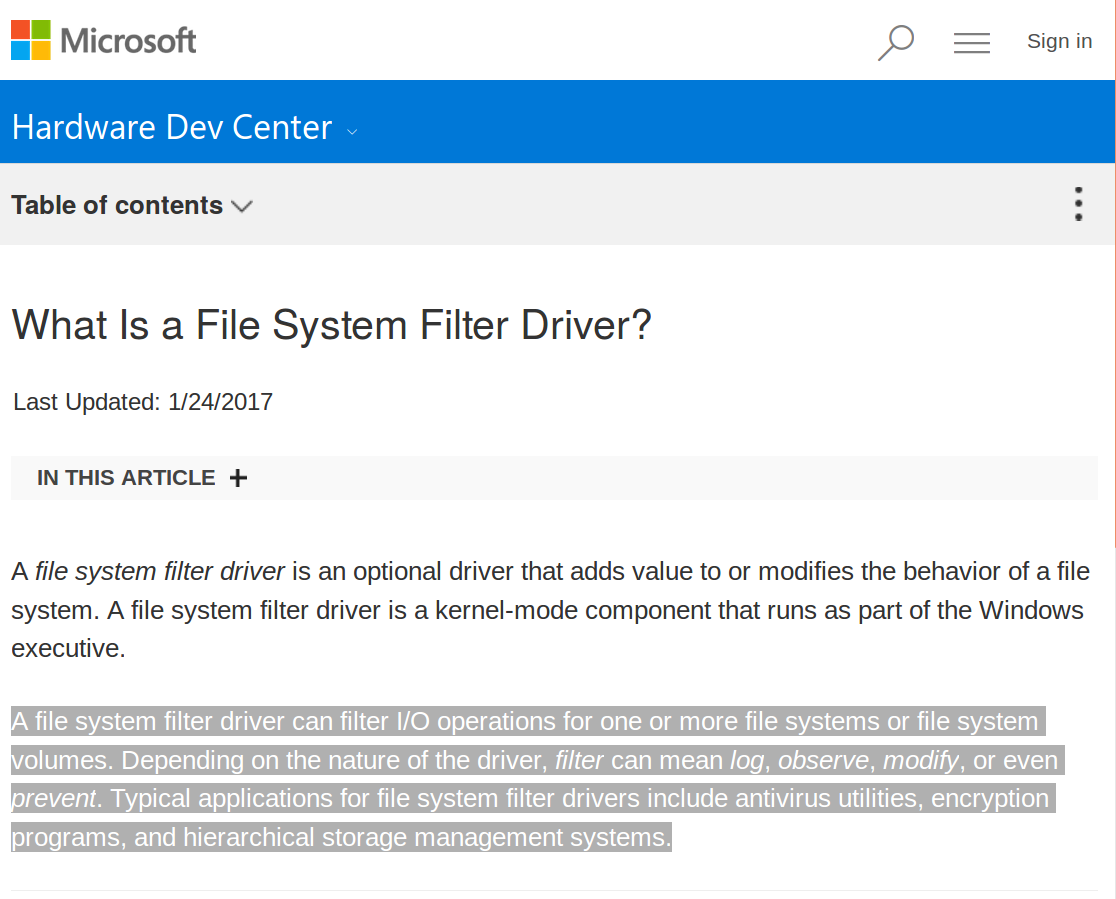
\includegraphics[height=0.9\textheight]{filter-driver}
\end{frame}

\againframe<3>{hookingList}

\begin{frame}{changing library loading}
\begin{itemize}
    \item e.g. install new library --- or edit loader, but \ldots
    \vspace{.5cm}
    \item not everything uses library functions
    \item what if your wrapper doesn't work exactly the same?
        \begin{itemize}
        \item problem both for malware and anti-virus!
        \end{itemize}
\end{itemize}
\end{frame}

\againframe<4>{hookingList}

\begin{frame}{changing exception handlers?}
    \begin{itemize}
    \item mechanism on DOS
    \item track what old exception handler does
    \item ``tunneling'' technique --- find the original, call it instead
    \end{itemize}
\end{frame}

\begin{frame}{other holes in behavior blocking}
    \begin{itemize}
    \item if in library: don't use library function
        \begin{itemize}
        \item e.g. copy of ``clean'' library
        \item e.g. statically linked
        \end{itemize}
    \item generally: multiple ways to do things?
        \begin{itemize}
        \item like VM problem: was something missed?
        \end{itemize}
    \vspace{.5cm}
    \item e.g.. file modifications blocked?
    \item just acccess the disk directly
    \end{itemize}
\end{frame}

\begin{frame}{attacking antivirus (2)}
    \begin{itemize}
    \item mechanisms other than hooking
    \item just directly modify it
        \begin{itemize}
        \item example: IDEA.6155 modifies database of scanned files
        \end{itemize}
    \item preserve checksums
        \begin{itemize}
        \item example: HybrisF preserved CRC32 checksums of infected files
        \item some AV software won't scan again
        \end{itemize}
    \end{itemize}
\end{frame}

\begin{frame}{not just hiding/interfering}
    \begin{itemize}
    \item our model of malware --- runs when triggered
    \item reality: sometimes keep on running
        \begin{itemize}
        \item evade active detection
        \item spread to new programs/files as created/run
        \end{itemize}
    \item call \myemph{resident}
    \end{itemize}
\end{frame}

\begin{frame}{spreading in memory}
    \begin{itemize}
    \item hook to hide virus file
    \item not just hiding virus --- propogate!
    \item example: infect any new files
    \item example: reinfect ``repaired'' files
    \end{itemize}
\end{frame}

\section{conclusion}

% FIXME: conclusion

\begin{frame}{armored viruses}
    \begin{itemize}
    \item ``encrypted'' viruses
        \begin{itemize}
        \item not strong encryption --- key is there!
        \end{itemize}
    \item self-changing viruses:
    \begin{tikzpicture}
    \begin{scope}[start chain=going right,node distance=2mm]
    \tikzset{
        every node/.style={font=\small,join,on chain},
        every join/.style={thick,Latex-Latex},
    }
    \node {encrypted};
    \node {oligiomorphic};
    \node {polymorphic};
    \node {metamorphic};
    \end{scope}
    \end{tikzpicture}
    \end{itemize}
\end{frame}

\begin{frame}{anti-debugging, tunnelling, etc.}
    \begin{itemize}
    \item anti-debugging/virtualisation/goat
        \begin{itemize}
        \item evade various ``\myemph{run it and check}'' techniques
        \end{itemize}
    \item tunnelling
        \begin{itemize}
        \item evade \myemph{behavior-blocking/detection}
        \end{itemize}
    \item stealth
        \begin{itemize}
        \item ``hook'' system operations (like antivirus)
        \item hide modified files, malware processes, etc.
        \end{itemize}
    \item retrovirus
        \begin{itemize}
        \item deliberately break antivirus software
        \end{itemize}
    \item memory residence
        \begin{itemize}
        \item infect running OS/programs, not just files
        \item antivirus needs to kill running virus code
        \end{itemize}
    \end{itemize}
\end{frame}

\section{Backup slides}
\begin{frame}{real signatures: ClamAV}
\begin{itemize}
\item ClamAV: open source email scanning software
\item signature types:
    \begin{itemize}
    \item hash of file
    \item hash of contents of segment of executable
        \begin{itemize}
        \item built-in executable, archive file parser
        \end{itemize}
    \item fixed string
    \item basic regular expressions
        \begin{itemize}
        \item wildcards, character classes, alternatives
        \end{itemize}
    \item more complete regular expressions
        \begin{itemize}
        \item including features that need more than state machines
        \end{itemize}
    \item meta-signatures: match if other signatures match
    \item icon image fuzzy-matching
    \end{itemize}
\end{itemize}
\end{frame}

\begin{frame}<1>[label=antiVirusTech]{anti-virus techniques}
    \begin{itemize}
    \item last time: \myemph<2,5>{signature-based detection}
        \begin{itemize}
        \item regular expression-like matching
        \item snippets of virus(-like) code
        \end{itemize}
    \item \myemph<3>{heuristic detection}
        \begin{itemize}
        \item look for ``suspicious'' things
        \end{itemize}
    \item \myemph<4>{behavior-based detection}
        \begin{itemize}
        \item look for virus activity
        \end{itemize}
    \item not explicitly mentioned: \myemph<5>{producing signatures}
        \begin{itemize}
        \item manual? analysis
        \end{itemize}
    \item not explicitly mentioned: ``disinfection''
        \begin{itemize}
        \item manual? analysis
        \end{itemize}
    \end{itemize}
\end{frame}

\subsection{heuristic case study}

\begin{frame}{example heuristics: DREBIN (1)}
    \begin{itemize}
    \item {\small from 2014 research paper on Android malware: Arp et al, ``DREBIN: Effective and Explainable Detection of Android Malware in Your Pocket''}
    \item features from applications (\myemph{without running}):
        \begin{itemize}
        \item hardware requirements
        \item requested permissions
        \item whether it runs in background, with pushed notifications, etc.
        \item what API calls it uses
        \item network addresses
        \end{itemize}
    \item detect \myemph{dynamic code generation} explicitly
    \item statistics (i.e. machine learning) to determine score
    \end{itemize}
\end{frame}

\begin{frame}{example heuristics: DREBIN (2)}
    \begin{itemize}
    \item advantage: Android uses Dalvik bytecode (Java-like)
        \begin{itemize}
        \item high-level ``machine code''
        \item much easier/more useful to analyze
        \end{itemize}
    \item accuracy?
        \begin{itemize}
        \item tested on 131k apps, $94$\% of malware, $1$\% false positives
        \item versus best commercial: $96$\%, $<0.3$\% false positives
            \begin{itemize}
            \item (probably has explicit patterns for many known malware samples)
            \end{itemize}
        \end{itemize}
    \item \ldots but
        \begin{itemize}
        \item statistics: training set needs to be typical of malware
        \item cat-and-mouse: what would attackers do in response?
        \end{itemize}
    \end{itemize}
\end{frame}
